\newpage
\noindent
\textbf{Beispiel 2}\\ \\
a)\\ \\
\begin{figure}[h]
	\centering
	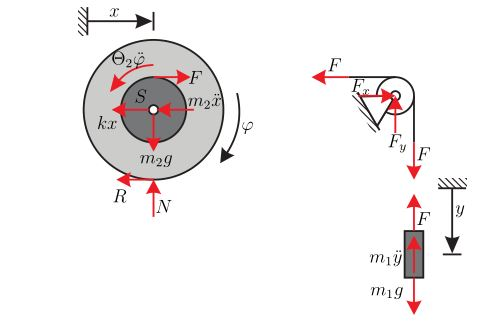
\includegraphics[width=10cm]{tikz/13_05_2016_2a}
\end{figure}
\newline
b)\\ \\
Kräftegleichgewicht der Trommel in der y-Richtung:
\[
	N - m_2g = 0
\]
c)\\ \\
Impuls- und Drehimpulsbilanz der Trommel:
\begin{align*}
	F - R - kx - m_2\ddot{x} &= 0 \\
	r_iF + r_aR - \Theta_2\ddot{\varphi} &= 0
\end{align*}
d) \\ \\
Impulsbilanz des Blockes in y-Richtung:
\[
	m_1g - F - m_1\ddot{y} = 0
\]
e)\\ \\
Da Geschwindigkeit im Punkt M gleich $0$ ist, gilt folgender Zusammenhang für den Schwerpunkt S
\begin{align*}
	\dot{x} &= r_a\dot{\varphi} \\
	\ddot{x} &= r_a\ddot{\varphi}
\end{align*}
\begin{figure}[h]
	\centering
	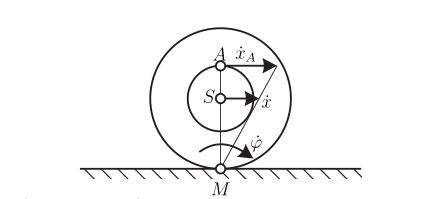
\includegraphics[width=10cm]{tikz/13_05_2016_2e}
\end{figure}
\newpage
\noindent
f)\\ \\
Zusammenhang:
\begin{align*}
	\dot{y} &= (r_i + r_a)\dot{\varphi} \\
	\ddot{y} &= (r_i + r_a)\ddot{\varphi}
\end{align*}
Dieser Zusammenhang ist aber nur dann gültig, wenn das Seil nicht ausgedehnt ist, da in diesem Fall $\dot{y} = \dot{x}_A$ gilt.\\ \\
g)\\ \\
Aus der Impulsbilanz der Trommel folgt
\[
	F = m_2\ddot{x} + R + kx
\]
Setzt man dies in die Drehimpulsbilanz ein und formt diese nach R um, erhält man
\[
	R = \frac{-m_2r_i\ddot{x} + \Theta_2\ddot{x} - kxr_i}{r_i + r_a}
\]
Rückeingesetzt ergibt das 
\[	
	F = m_2\ddot{x} + \frac{-m_2r_i\ddot{x} + \Theta_2\ddot{x} - kxr_i}{r_i + r_a} + kx
\]
Setzt man nun alle bekannten Größen in die Impulsbilanz des Blockes ein, erhält man schließlich
\[
	m_1g - m_2\ddot{x} - \frac{-m_2r_i\ddot{x} + \Theta_2\ddot{x} - kxr_i}{r_i + r_a} - kx - m_1(r_i + r_a)\ddot{\varphi} = 0
\]
Formt man nun diese Gleichung auf $\ddot{\varphi}$ um, ergibt sich
\[
	\ddot{\varphi} = \frac{- m_2\ddot{x}r_a + m_1g(r_i + r_a) - kxr_a}{m_1(r_i + r_a)^2 + \Theta_2}
\]
Dies in $\ddot{x}$ eingesetzt, folgt
\[
	\ddot{x} = \frac{-m_2\ddot{x}r_a^2 + m_1gr_a(r_i + r_a) - kxr_a^2}{m_1(r_i + r_a)^2 + \Theta_2}
\]
Somit folgt die Bewegungsgleichung
\begin{align*}
\ddot{x}\left( 1 + \frac{m_2r_a^2}{m_1(r_i + r_a)^2 + \Theta_2}\right) &= \frac{m_1gr_a(r_i + r_a) - kxr_a^2}{m_1(r_i + r_a)^2 + \Theta_2} \\
\ddot{x}\left(\frac{m_1(r_i + r_a)^2 + \Theta_2 + m_2r_a^2}{m_1(r_i + r_a)^2 + \Theta_2}\right)  &= \frac{m_1gr_a(r_i + r_a) - kxr_a^2}{m_1(r_i + r_a)^2 + \Theta_2} \\
\end{align*}
zu
\[
\ddot{x} = \frac{m_1(r_i + r_a)gr_a - kxr_a^2}{m_1(r_i + r_a)^2 + m_2r_a^2 + \Theta_2}
\]